\subsection{Modultest database}
\label{ssec: Modultest database}
Den lokale hosting medførte at vi kunne holde øje med databasens udformningen, samt den gemte data, gennem Microsoft azure datastudie.\\

\noindent For at teste DAL funktioner og dens forbindelse til databasen, oprettes først et DAL objekt med en context som indeholder en korrekt connectionstring.

\noindent Til test hvor der skal læses fra databasen, kaldes den passende DAL funktion, hvorefter den hentede information udskrives på konsolen. Korrektheden af det fundne tjekkes med data studie.

\noindent Til test hvor der skal indsættes data i databasen oprettes der objekter af den korrekte type hvorefter DAL funktioner til indsættelse kaldes. Korrektheden af de indsatte data kan herefter tjekkes med datastudie.
Et eksempel på dette kan ses på \autoref{fig:SaveGame-test} herunder.
Her oprettes et GameDTO objekt, gamesave.\\
Gamesave opsættes til ”Gamer1”, med navnet ”My First Run”, hvorefter der tilføjes yderligere data. Det overskrevne save er ”NewGame1”, som her har id 1.

\begin{figure}[H]
\centering
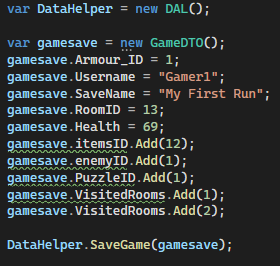
\includegraphics[width = 0.5\textwidth]{02-Body/Images/DAL-Database/DB-Test.png}
\caption{Kode til test af SaveGame, hvor der oprettes et nyt save som overskriver det gamle save med saveID 1}
\label{fig:SaveGame-test}
\end{figure}

\noindent På \autoref{fig:datastudie-før} herunder ses et screenshot fra datastudie hvor de 5 saves til ”Gamer1” kan ses.
Det noteres at alle saves er "tomme" og starter i rum 1.

\begin{figure}[H]
\centering
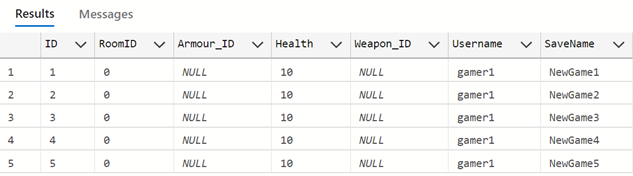
\includegraphics[width = \textwidth]{02-Body/Images/DAL-Database/DatastudieFørIndsættelse.png}
\caption{Screenshot fra datastudie før opdatering af save hvor de 5 ens "tomme" saves kan ses}
\label{fig:datastudie-før}
\end{figure}

Herefter køres programmet fra \autoref{fig:SaveGame-test}, og vi kan nu se ændringerne i databasen.
Det noteres at SaveName og de andre attributter i \autoref{fig:datastudie-efter} nu er opdateret korrekt efter koden.

\begin{figure}[H]
\centering
\includegraphics[width = \textwidth]{02-Body/Images/DAL-Database/DataStudieEfterIndsættelse.png}
\caption{Sceenshot af datastudie efter overskrivning af save 1. Her er saveID 1 opdateret til nu at hedde "My First Run" og health og roomID er ændret korrekt, så det passer med det indsatte}
\label{fig:datastudie-efter}
\end{figure}

\noindent De øvrige tilhørende lister til det gemte save er også opdateret med korrekte værdie. Dette kan også ses på \autoref{fig:Datastudie-ekstra} herunder.

\begin{figure}[H]
\centering
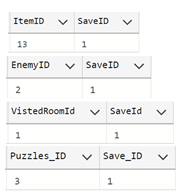
\includegraphics[width = 0.4\textwidth]{02-Body/Images/DAL-Database/Lister.png}
\caption{Sceenshot af datastudie efter overskrivning af save 1 med ekstra tabeller som referer til det rigtige saveID}
\label{fig:Datastudie-ekstra}
\end{figure}

I ovenstående sekvens ses det at data bliver indsat korrekt i databasen og funktionen er altså godtkendt.
I det tekniske bilag \textbf{AFSNIT REF HER} findes en tabel over godkendelse af DAL-Db forbindelsen.\\

Den ovenstående modultest er generelt godkendet da alle funktioner opfører sig som forventet, i og med at der hentes og gemmes korrekt i databasen. Med alle funktioner testet og godkendt er DAL-database forbindelsen klar til at blive integreret med resten af systemet.
